Her følger en beskrivelse af kildekode fil strukturen og hvordan denne omsættes til de forskellige enheder.

\subsection{Filstruktur}
På figur \ref{fig:filstruktur1} er filstrukturen vist for software implementeringen.
De er delt op i tre mapper: PC, CSS hovedenhed og X10 udtag.

\begin{figure}[!htb]
     {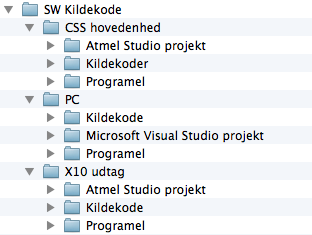
\includegraphics[width=\textwidth]{billeder/Filstruktur1}}
     \caption{Overordnet filstruktur}
     \label{fig:filstruktur1}
\end{figure}

I hver mappe ligger de rå kildekoder, et projekt i det tilhørende udviklingsprojekt og de rå programmer som bruges på hver platform, hhv. .exe og .hex til PC og CSS hovedenhed og X10 udtag.
I tabel \ref{table:Udviklingsprogrammer} er vist hvilke udviklingsværktøjer der er brugt til de forskellige platforme.

\begin{table}[htb]
	\caption{Udviklingsplatforme til software udviklingen}
	\centering
	\begin{tabular}{|c|c|}
		\hline 
		\textbf{Enhed} & \textbf{Udviklingsprogram} \\ 
		\hline 
		PC & Microsoft Visual Studio 2012 \\ 
		\hline 
		CSS hovedenhed & Atmel Studio 6.1 \\ 
		\hline 
		X10 udtag & Atmel Studio 6.1 \\ 
		\hline 
	\end{tabular} 
	\label{table:Udviklingsprogrammer}
\end{table}
